\chapter{BẢN VẼ SCHEMATIC}
\section{Các cụm chức năng trên bản vẽ schematic}

\subsection{Cụm nguồn động cơ}
\begin{figure}[H]
    \centering
    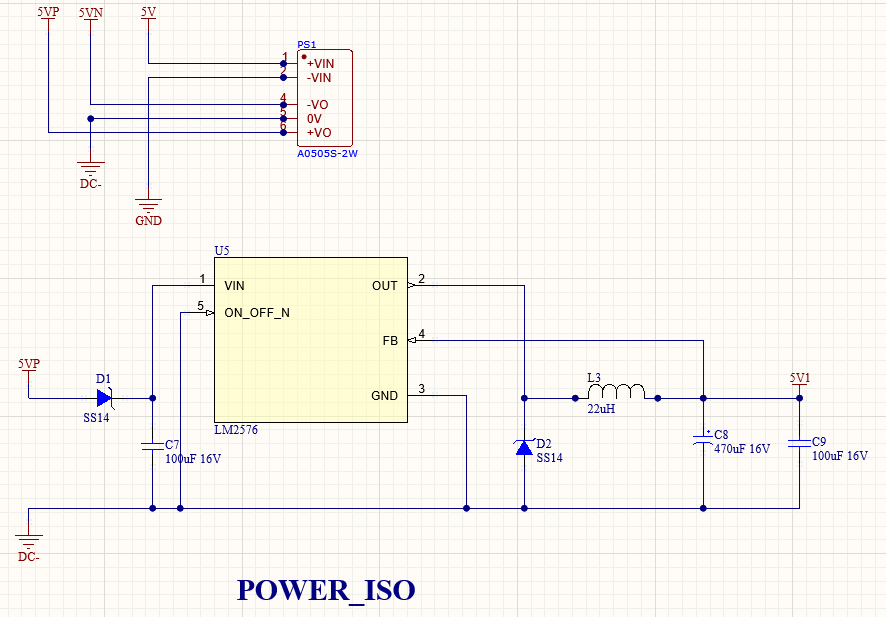
\includegraphics[width=1\textwidth]{pictures/power_iso.png}
\end{figure}
\begin{itemize}
    \item Ở cụm nguồn trên, sử dụng module nguồn cách ly DC-DC A0505S-2W để chuyển đổi nguồn và có 
    tác dụng cách ly điện áp. Cụ thể module nhận điện áp 5V ở đầu vào (chân +VIN) sau đó chuyển đổi 
    thành 2 nguồn 5VP và 5VN ở đầu ra (nguồn 5VP tương ứng với chân +VO và 0V, nguồn 5VN tương ứng với 2 chân -VO và 0V). Tuy nhiên dòng tải tối đa module này có thể cung cấp chỉ khoảng từ 400mA đến 500mA.
    \item Ngoài ra LM2576 là một IC điều chỉnh điện áp hạ áp, trong cụm chức năng này, IC LM2576 thực hiện lấy điện áp 5V từ đầu ra
    của module A0505S-2W làm điện áp đầu vào để ổn định điện áp ở mức 5V đồng thời cung cấp dòng lớn (3A), phù hợp cho yêu cầu của các tải phía sau.
\end{itemize}

\subsection{Cụm điều khiển động cơ}
\begin{figure}[H]
    \centering
    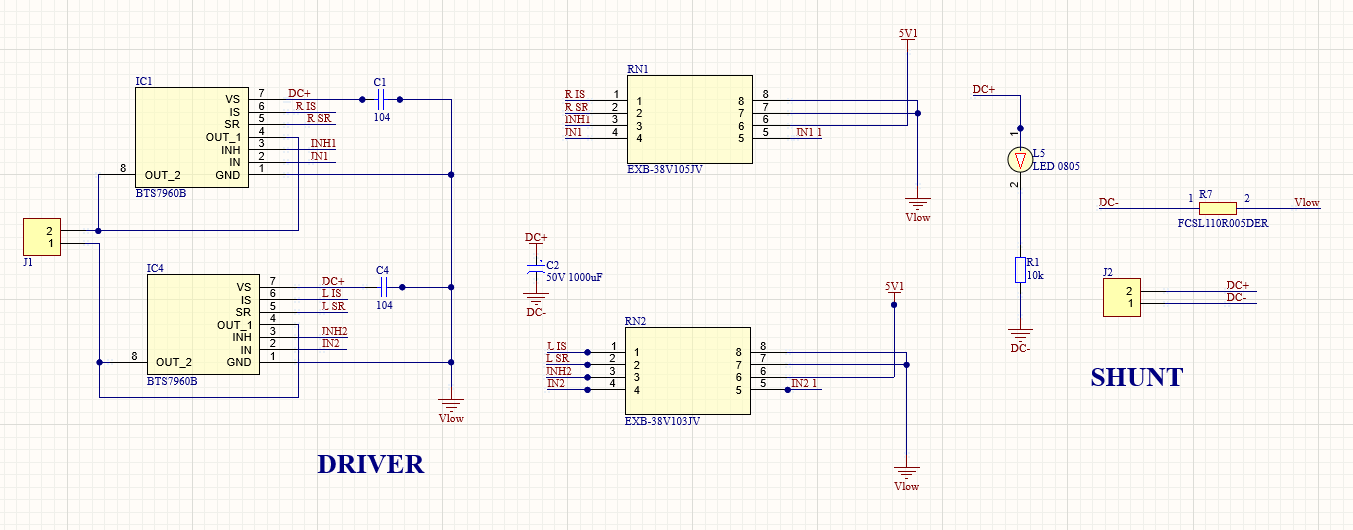
\includegraphics[width=1\textwidth]{pictures/driver.png}
\end{figure}
\begin{itemize}
    \item Trong cụm DRIVER sử dụng 2 IC BTS7960B để tạo thành một mạch cầu H điều khiển hướng quay và tốc độ động cơ bằng cách thay đổi trạng thái 2 chân INH và IN.
    \item RN1, RN2 (EXB-38V105JV): các mạng điện trở (resistor network) dùng để điều chỉnh tín hiệu điều khiển từ bộ vi điều khiển (MCU) xuống các chân INH và IN của BTS7960B.
    \item Tụ gốm C1 và C4 100nF để lọc nhiễu ở chân cấp nguồn DC+.
    \item Tụ lọc lớn C2 1000uF để ổn định nguồn DC+.
    \item Header J1 dùng để giao tiếp, nhận tín hiệu điều khiển từ MCU (INH1, INH2, IN1, IN2).
    \item Cụm trở SHUNT gồm 1 trở R7 (FCSL110R005DER): Đây là điện trở shunt có giá trị nhỏ (0.005 $\Omega$), dùng để đo dòng điện qua động cơ bằng cách đo điện áp rơi trên trở shunt R7). Giá trị đo được gửi về vi điều khiển để xử lý và gửi tín hiệu ngược lại cụm 
    DRIVER để điều khiển tốc độ động cơ.
\end{itemize}

\subsection{Cụm vi điều khiển MCU}
\begin{figure}[H]
    \centering
    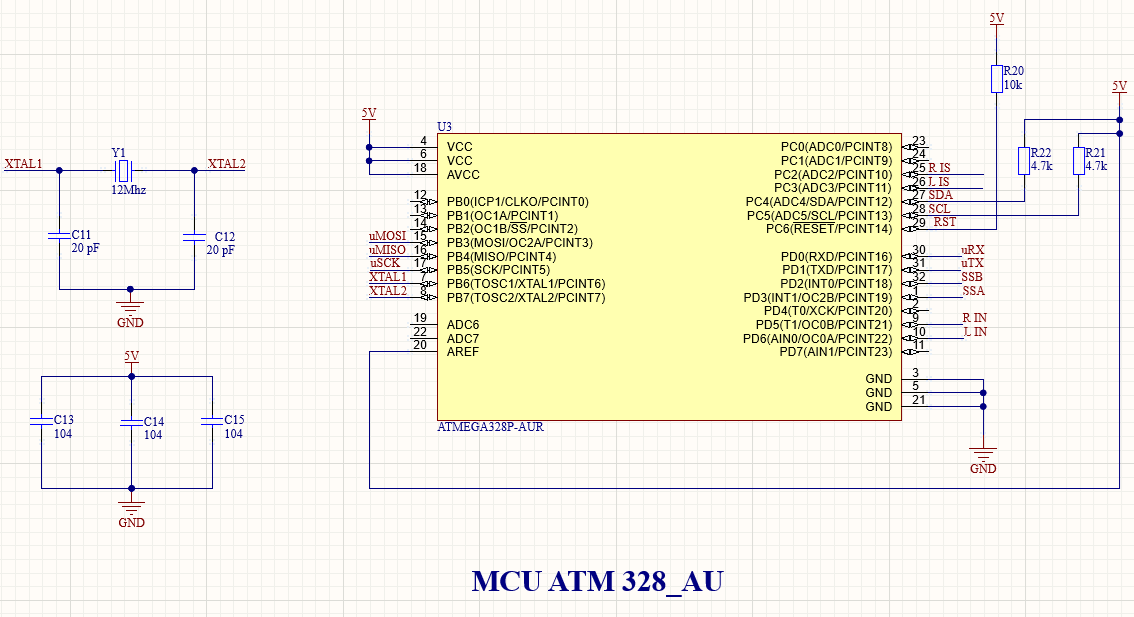
\includegraphics[width=1\textwidth]{pictures/mcu.png}
\end{figure}
\begin{itemize}
    \item Vi điều khiển được sử dụng trong schematic là ATMega328P-AUR, là một loại vi điều khiển 8-bit rất phổ biến, được sử dụng rộng rãi trong các dự án nhúng.
    Sử dụng kiến trúc RISC giúp tăng tốc độ thực thi và giảm kích thước bộ vi xử lý.
    \item Hỗ trợ nhiều chân GPIO I/O có thể được cấu hình để làm đầu vào, đầu ra kỹ thuật số hoặc hỗ trợ cho gioa tiếp SPI, I2C, UART, \dots
    \item Điện áp hoạt động hỗ trợ trong khoảng lớn, linh hoạt trong các dự án.
    \item Trong bản thiết kế Schematic trên, MCU thực hiện các loại giao tiếp I2C (qua 2 điện trở kéo lên R20, R21 vào 2 chân SDA, SCL), giao tiếp SPI (uMOSI, uMISO), UART (uRX, uTX)
\end{itemize}


\subsection{Cụm đọc tín hiệu Analog}
\begin{figure}[H]
    \centering
    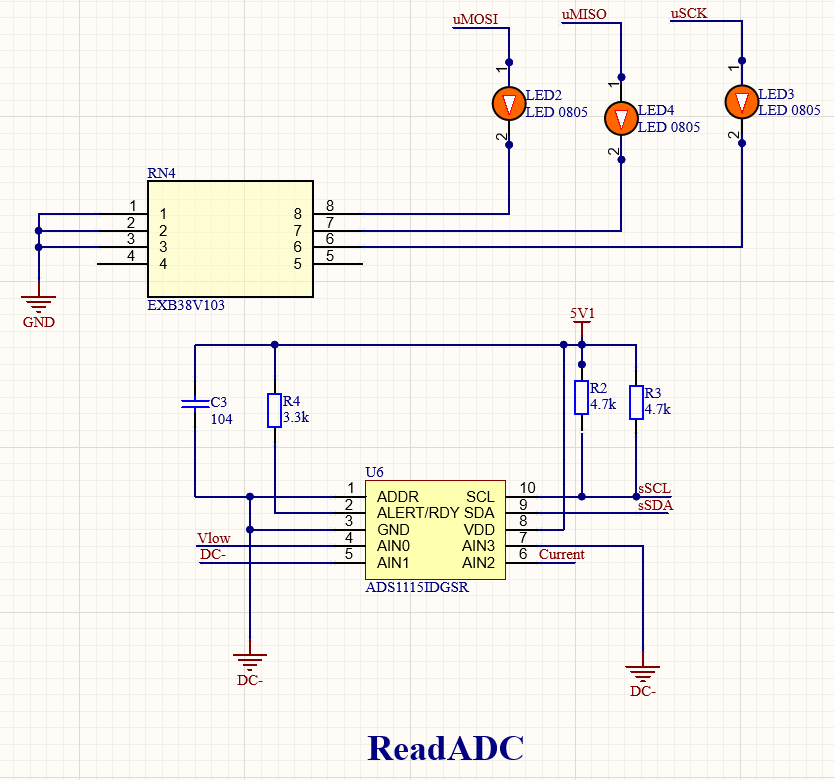
\includegraphics[width=0.9\textwidth]{pictures/readADC.png}
\end{figure}
\begin{itemize}
    \item IC chính sử dụng trong cụm này là ADS1115IDGSR, một bộ chuyển đổi ADC (Analog-to-Digital Converter) với độ phân giải 16 bit và giao tiếp I2C.
    Trong mạch, IC này chuyển các tín hiệu analog từ các chân AIN0, AIN1, AIN2 thành tín hiệu số, đây là các tín hiệu từ cụm trở shunt bao gồm điện áp rơi và dòng qua động cơ, chuyển đổi thành các tín hiệu số
    sau đó giao tiếp với vi điều khiển thông qua giao tiếp I2C (qua các chân sSCL, sSDA)
    \item Các điện trở pull-up R2, R3 cho các chân SCL, SDA đảm bảo giao tiếp I2C ổn định.
    \item Tụ gốm C3 104 giúp lọc nhiễu cho IC.
\end{itemize}


\subsection{Cụm cách ly}
\begin{figure}[H]
    \centering
    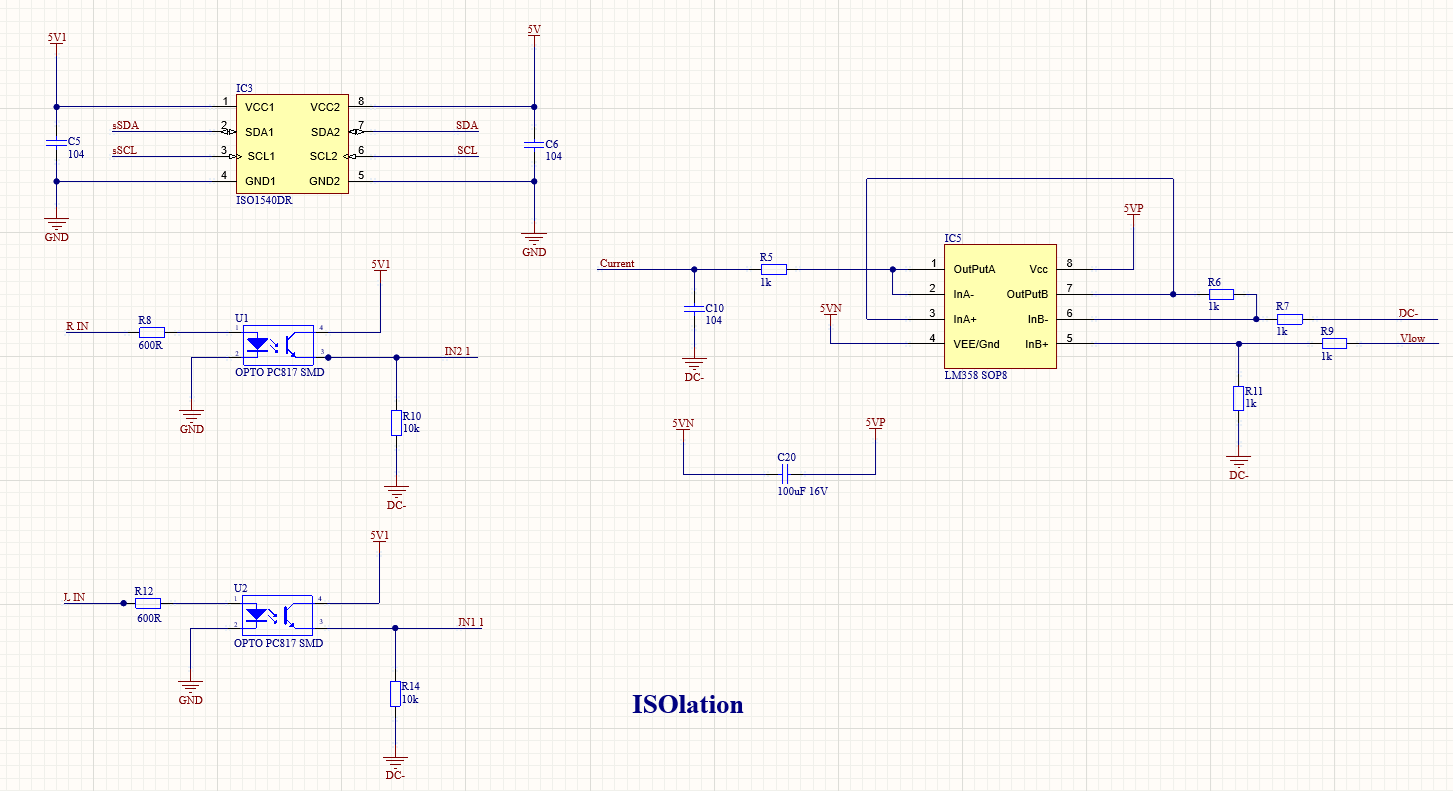
\includegraphics[width=1\textwidth]{pictures/isolation.png}
\end{figure}
Cụm ISOlation trong sơ đồ có chức năng chính là cách ly tín hiệu giữa các phần của mạch để ngăn chặn nhiễu, bảo vệ mạch.
\begin{itemize}
    \item Khối cách ly I2C (ISO1540DR): Đây là IC cách ly tín hiệu I2C. 2 chân VCC1 và VCC2 cấp nguồn cho 2 phía của IC, cách ly hoàn toàn SDA1/SCL1 (kết nối với cụm ReadADC) và SDA2/SCL2(kết nối với MCU).
    \item Khối cách ly tín hiệu dòng/điện áp (OPTO PC817): là các optpcoupler (quang cách ly), giúp cách ly tín hiệu analog. Cách hoạt động: Khi dòng chạy qua LED bên trong optocoupler (từ 2 chân R IN, L IN trên MCU), ánh sáng phát ra kích hoạt transistor bên trong (chân 3 và 4), dẫn dòng qua đầu ra (đầu ra là 2 chân LN1 1 và LN2 1, nhằm điều khiển cầu H ở cụm DRIVER). 
    Tín hiệu được truyền mà không có kết nối điện trực tiếp, giúp cách ly hoàn toàn hai phía mạch.
    \item Khối khuếch đại và đo tín hiệu dòng (LM358 SOP8): l 1à op-amp (Operational Amplifier) hoạt động ở chế độ khuếch đại vi sai. Cách hoạt động: Nhận tín hiệu Vlow và DC- từ cụm trở Shunt vào chân InB+ và InB-, OutputB được đưa vào InA+ của Op-Amps thứ 2, tín hiệu đầu ra OutputA là Current (dòng đã được khuếch đại) và tín hiệu analog đi vào chân AIN2 tương ứng trên cụm ReadADC.
    \item 
\end{itemize}

\section{Bản vẽ schematic hoàn chỉnh}
\begin{figure}[H]
    \centering
    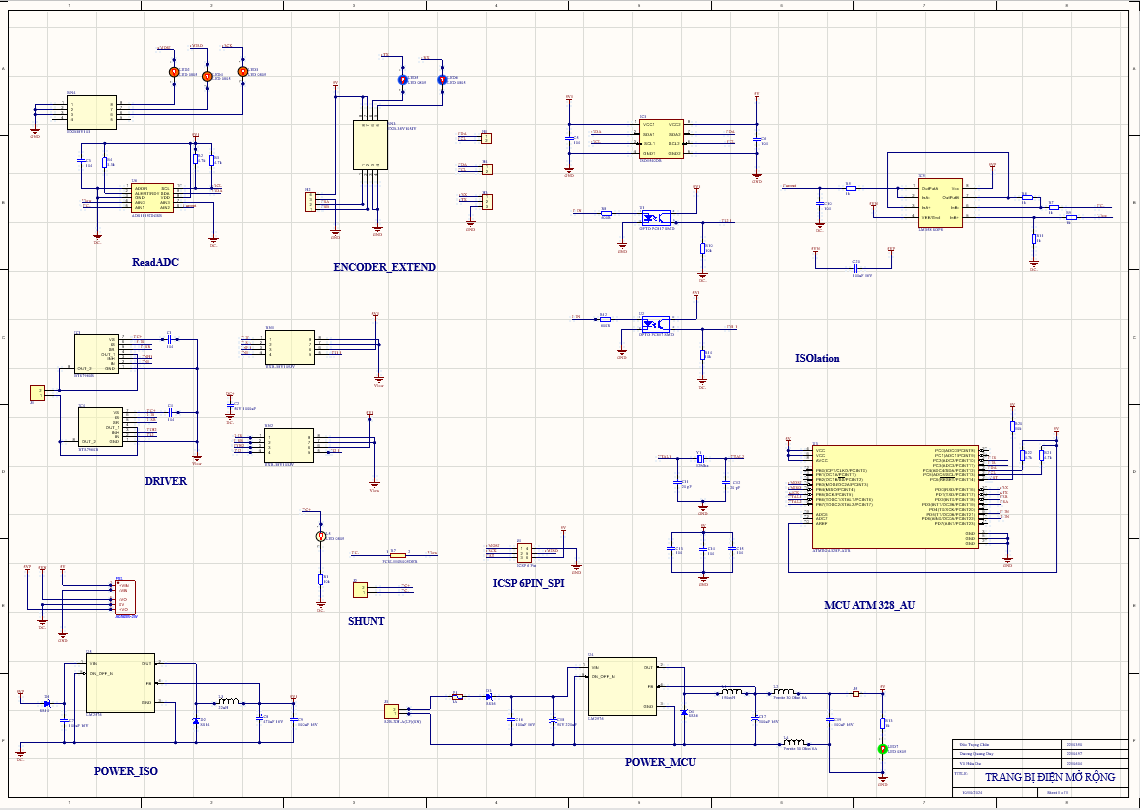
\includegraphics[width=1\textwidth]{pictures/ISO_current.png}
    \caption{Bản vẽ schematic hoàn chỉnh}
\end{figure}
\cleardoublepage
